\documentclass{standalone}
\usepackage{tikz}
\begin{document}

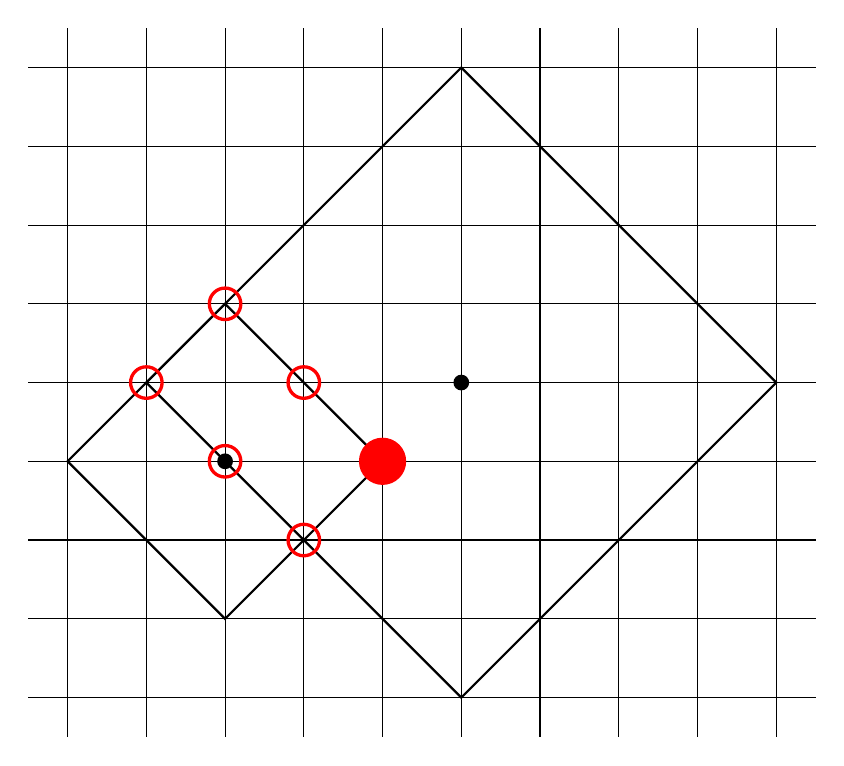
\begin{tikzpicture}
	\newcommand\overhang{0.5};
	\newcommand\xmin{-5};
	\newcommand\xmax{4};
	\newcommand\ymin{-4};
	\newcommand\ymax{4};
	\foreach \i in {\xmin,...,\xmax} {
		\draw (\i, \ymin-\overhang) -- (\i, \ymax+\overhang);
	}
	\foreach \i in {\ymin,...,\ymax} {
		\draw (\xmin-\overhang, \i) -- (\xmax+\overhang, \i);
	}
	\fill (0,0) circle (.1);
	\draw[thick] (0,4) -- (4,0) -- (0,-4) -- (-4,0) -- cycle;
	\fill (-3,-1) circle (.1);
	\draw[thick] (-3,1) -- (-1,-1) -- (-3,-3) -- (-5,-1) -- cycle;
	\fill[red] (-1,-1) circle (.3);
	\draw[red,very thick] (-3,-1) circle (.2);
	\draw[red,very thick] (-2,0) circle (.2);
	\draw[red,very thick] (-2,-2) circle (.2);
	\draw[red,very thick] (-4,0) circle (.2);
	\draw[red,very thick] (-3,1) circle (.2);
\end{tikzpicture}

\end{document}
